%!TEX root = project.tex

\chapter*{About this project}
\paragraph{Abstract}
Competitive online gaming has seen a significant increase in popularity in recent times, whether watching or participating, competitive games can consume a large portion of our free time. Organising tournaments require organisation and rules. To ensure the rules are upheld require some form of administration from a system or individual. Issues can occur when an individual is responsible for managing these tournaments, for example, if a tournament has a fixed schedule but the person responsible for managing the tournament is unavailable, then the tournament game must be postponed. Administrators are also required to ensure matchmaking fairness between teams which can be very time consuming and inefficient.

\paragraph{Authors}
Ethan Horrrigan



\chapter{Introduction}
Competitive online gaming has seen a significant increase in popularity in recent times. The estimated global esports audience was estimated at 335 million people in 2017 generating a revenue of more than \$900M with an estimated growth of over \$1600M in 2021.~\cite{sjoblom2019esports} Yuri Seo and Sang-Uk Jung ~\cite{seo2016beyond} outlined why people play or spectate competitive games. The main factors include entertainment and gaining a better understanding of a game. Whether spectating or participating, competitive games can consume a large portion of our free time. Organising matches need some form of administration to ensure rules are upheld. A person or system is usually responsible for this. Issues occur when an individual is responsible for managing these games, for example, if a match has a fixed schedule but the person responsible for managing the game is unavailable, then the tournament game must be postponed. Administrators are also required to ensure matchmaking fairness between teams which can be very time consuming and unpredictable. These factors are the reason why I've developed a service for people to manage and administrate their events or matches.

\chapter{Context}
\begin{itemize}
	\item This project aims to create a platform for people to manage and compete in online custom games.
	\item The core objectives are to develop a web application for people to create and find custom games and to handle handle matchmaking for these games.
	\item Briefly list each chapter / section and provide a 1-2 line description of what each section contains.
	\item List the resource URL (GitHub address) for the project and provide a brief list of the main elements at the URL.
\end{itemize}

\section{League of Legends}
NOTE: Relevant information to my solution.
NOTE: Remove usless information.
NOTE: How tournaments work (Online)
League of Legends is a free-to-play multiplayer online battle arena (MOBA). A team consists of five players on either side. The map consists of three lanes (Top lane, Middle lane and Bottom lane) and a Jungle on each side of the map. Each player is responsible for fulfilling these lanes and controlling their characters (champions). The main objective of the game is to defeat the enemy nexus (base). Players can accomplish this by fighting the opposition in solo fights or team fights. Players can purchase items throughout the game to strengthen their character, all players gain experience and gold by killing minions and other players. This is the main source of income for players to upgrade their items. Players can build damage or resistances depending on what characters the enemies are playing.
League of Legends is heavily Team-Based. The skill level of a team is an important condition for team effectiveness. The team's skill level is based on the combination of skills and attributes of its members.

\section{Rating}
Bronze, Silver, Gold, Platinum, Diamond, Master, Grandmaster and Challenger. All tiers have four divisions within each tier up until master. A division contains 100 league points (LP) that players gain or lose depending on match outcome. 78.31\% of the player base are either bronze, silver or gold. Whereas only 0.02\% of players are challenge
\section{Custom Games}
In most online multiplayer games, custom lobbies can be created allowing people to
Players also acquire ranks, which are broken up into several tiers: Iron, r tier \cite{kou2016ranking}.

\begin{center}    
	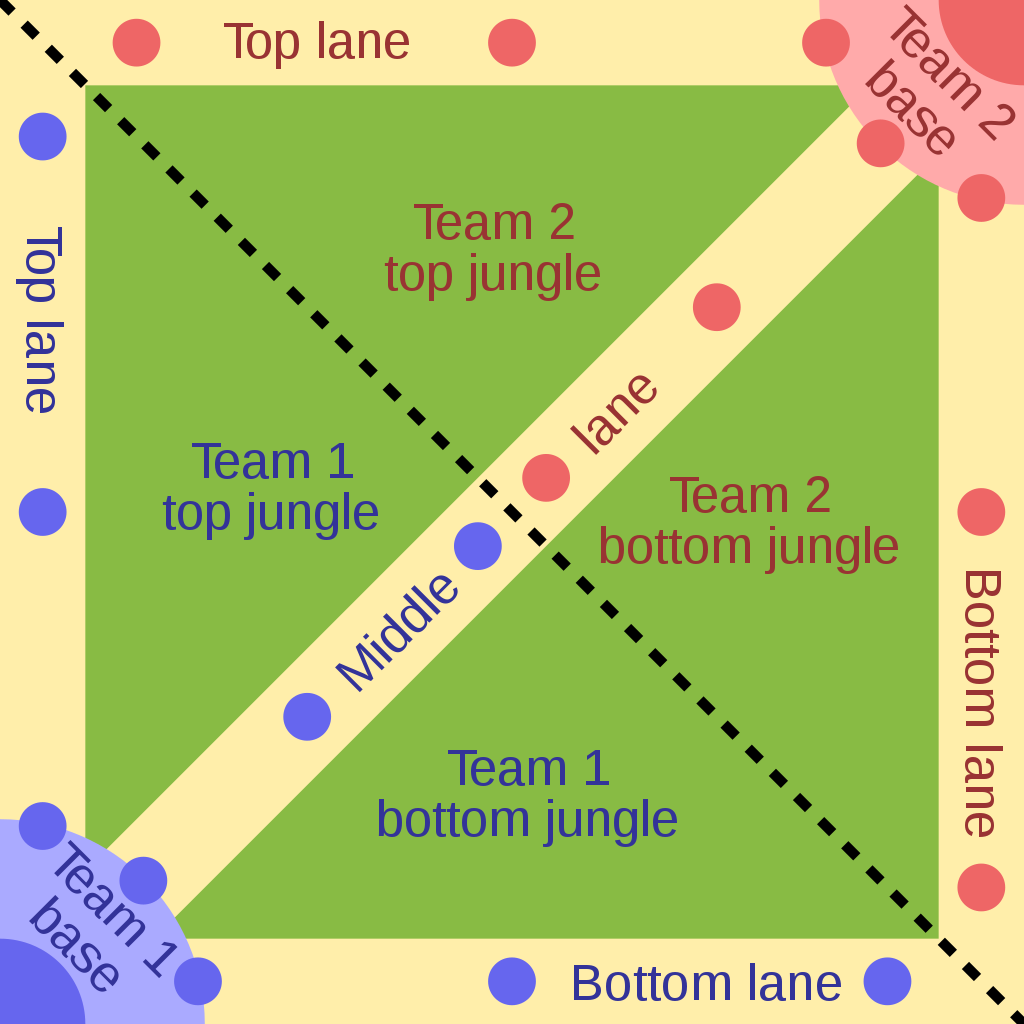
\includegraphics[width=8cm,height=4.3cm,keepaspectratio]{img/Map.png}
\end{center}
\clearpage

League of Legends is heavily Team-Based. The skill level of a team is an important condition for team effectiveness. The team's skill level is based on the combination of skills of its members.
A team consists of five players on either side. Each player is responsible for controlling their characters (champions) to defeat the enemy in solo duels and/or contriubte in team fights with the end goal of destroying the nexus. Players can purchase items throughout the game to strengthen their character, all players gain experience and gold by killing minions and other players. This is the main source of income for players to upgrade their items. Players can build damage or resisitances depending on the enemies character.

\subsection{Competitive Tournaments}

\subsection{More filler}

\section{Filler}


\chapter{Methodology}
\section{Development Methodology}
Project meetings were established at the beginning of development, Initial meetings consisted of brainstorming and considering project ideas. During this period, I conducted research on various technologies that could possibly be used throughout the project. I began development once the project was defined and understood what technologies were suitable for use throughout. Every week I would meet with my supervisor and discuss what has been implemented in the past week and what I will work on for the upcoming week. I took an iterative approach in the development of this project so I could see significant developments in the project.
\section{Testing}
I opted to use System Testing
I opted to use System Testing as the main type of testing for the project as this suited my workflow. I wanted to implement the functionality of client-side elements before testing. Unit tests were carried out near completion of development on individual components for both server-side and client-side. Jasmine and Karma was the framework used to test the functionality of web components.

TALK ABOUT SELENIUM
\begin{center}    
	
\includegraphics[width=8cm,height=3.3cm,keepaspectratio]{img/Jasmine_and_Karma.png}
\end{center}
Python’s Unittest was used to test server-sided functions ensuring that both HTTP Requests and the Matchmaking algorithm operated as expected.
\begin{center}    
	
\includegraphics[width=8cm,height=3.3cm,keepaspectratio]{img/Unittest.png}
\end{center}
End to end testing (e2e) was used to test the interactions and relationships between the backend and the presentation layer of the application. E2e testing was a great way to ensure that the components of the application worked together cohesively and also the application functioned correctly at a high-level overview. I concluded that unit tests were not sufficient enough, as unit tests only tested isolated elements of my project. I needed to test how the application's components operated as a combination. E2e testing was the best way to accomplish this.
Test cases were generated by scenarios in the following ways:~\cite{bai2001distributed}
\begin{itemize}
	\item (1) Identify the input data that meet the conditions associated with the component based on different testing techniques (e.g. unit tests).
	\item (2) Determine the expected results from input data. 
\end{itemize}
The main way I generated test cases was based on application usage, e.g., one component can be affected by several conditions, and each condition can be satisfied by multiple data. For example, the registration element may have input data such as username, summoner name and password. Therefore, the conditions for this test case include
\begin{itemize}
	\item 1) Valid username; 
	\item 2) Valid summoner name; 
	\item 3) Valid password;
\end{itemize}
The first test case satisfied these inputs and then the second test case took the exact input from the first scenario proving that duplicate usernames cannot be inserted into the database.

\section{Source Control}
GitHub was used for source control and project management. Initially, I was using Trello for task management but this quickly became complicated to associate updates with unfinished tasks of the project. Therefore I changed the projects task management to GitHub’s Issues section. I posted issues for any viable element that needed to be implemented into the project and when one of these elements were complete I would close the corresponding issue on GitHub. Each issue was categorized with tags depending on the type. These tags include:
\begin{itemize}
	\item To-do: Tasks that have yet to be implemented.
	\item Tests: Types of tests that have been or need to be carried out.
	\item Bugs: Issues or bugs that occurred throughout the project and how they were solved.
	\item In progress: In progress are tasks that are currently being implemented.
	\item Completed: Finished tasks.
	\item Enhancement: When a completed part of the project has been upgraded, changed or removed.
\end{itemize}
This method of task management proved to be a lot more manageable compared to my previous method of using Trello. I could easily compare my current tasks to my commits on GitHub. Anytime I had implemented a significant change or addition to my project, I would perform commit it to through git and push the change.

\section{Technologies Selection Criteria}
The primary development environment used throughout the project was Visual Studio Code, The main reasons why I chose this environment is because it supports debugging, Git control, syntax highlighting, intelligent code completion and for its customisability. Both Frontend and backend of the project were developed in this environment.
I used Angular which is an open-source web application framework led by the Angular Team at Google. The reasoning behind choosing Angular is because I wanted the project to be a web application as compared to a hybrid application, Angular seemed to be the most viable framework for this application.
When researching options for the database server, the two main options were python and flask or using MEAN stack (Mongo, Express.js, Angular and Node). I wanted the database to be a relational instead of using a NoSQL database, so a NoSQL database did not suit. I also wanted to use a technology that I'm not familiar with. These factors
\par
\begin{itemize}
	\item Agile / incremental and iterative approach to development. Planning, meetings.
	\item What about validation and testing? Junit or some other framework.
	\item If team based, did you use GitHub during the development process.
	\item Selection criteria for algorithms, languages, platforms and technolo-gies.
\end{itemize}
Check out the nice graphs in Figure \ref{tikz:graphs}, and the nice diagram in Figure \ref{tikz:mydiagram}.

\begin{figure}
	\centering
	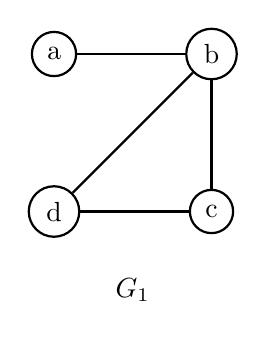
\begin{tikzpicture}
	\begin{scope}[every node/.style={circle,thick,draw}]
	\node (a) at (0,2) {a};
	\node (b) at (2,2) {b};
	\node (c) at (2,0) {c};
	\node (d) at (0,0) {d};
	\end{scope}
	\begin{scope}[every edge/.style={draw=black,thick}]
	\path (a) edge (b);
	\path (b) edge (c);
	\path (b) edge (d);
	\path (c) edge (d);
	\end{scope}
	\node () at (1,-1) {$G_1$};
	\end{tikzpicture}
	\hspace{1.5cm}
	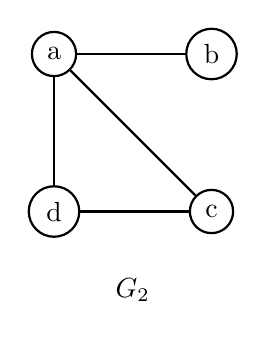
\begin{tikzpicture}
	\begin{scope}[every node/.style={circle,thick,draw}]
	\node (1) at (0,2) {a};
	\node (2) at (2,2) {b};
	\node (3) at (2,0) {c};
	\node (4) at (0,0) {d};
	\end{scope}
	\begin{scope}[every edge/.style={draw=black,thick}]
	\path (1) edge (2);
	\path (1) edge (3);
	\path (1) edge (4);
	\path (3) edge (4);
	\end{scope}
	\node () at (1,-1) {$G_2$};
	\end{tikzpicture}
	\caption{Nice pictures}
	\label{tikz:graphs}
\end{figure}


\begin{figure}
	\centering
	\begin{tikzpicture}[node distance=6cm]
	\node (a) [rect] {A Big Blue Block};
	\node (b) [oval, right of=a] {And His Oval Friend};
	\draw [line] (a) -- (b);
	\end{tikzpicture}
	\caption{Nice pictures}
	\label{tikz:graphs}
\end{figure}


\chapter{Technology Review}
\section{Angular}
Angular is an open-source web application framework led by the Angular Team at Google. It is often used for building Single Page Applications (SPA). What is a Single Page Application? In a web application, when you navigate to a different page, the entire page is reloaded, in a SPA, only the view of the content requested is reloaded. SPA provides a fluid experience for the user. A good example of a Single Page Application is Twitter. Since this application is a SPA, navigating between pages was smooth. A constant array of Routes is declared for every component.
\begin{minted}{typescript}
const routes: Routes = [
{ path: 'mypath', component: MyComponent}
{ path: 'mypath2', component: MyComponentTwo}
{ path: 'mypath3', component: MyComponentThree}
];
\end{minted}

\subsection{Why Angular?}

\begin{itemize}
	\item Components
\end{itemize}
Angular allows you to create components that provide functionality, styling and views.

\begin{itemize}
	\item Dynamic Routes
\end{itemize}
I could create unique URLs through Angulars ActivatedRoutes feature. I used this for viewing users profiles and particular match details. The URL parameters could also be accessed.
\newpage Example Button to view a match.
\begin{minted}{typescript}
//Typescript
{ path: 'match/:matchId', component: ViewMatchComponent},
\end{minted}
\begin{minted}{html}
 <!-- HTML -->
<a href="match/{{game.match_uuid}}" class="btn btn-primary">Join</a></li>
\end{minted}

\begin{itemize}
	\item Data Binding
\end{itemize}
Allows accessing of data from Typescript code to the html page view. This eliminates the process of implementing data binding myself.
Example:
\begin{minted}{typescript}
// TypeScript String Variable
myString: string = "Hello, World";

// Data Binding on the HTML Page
{{myString}}
\end{minted}

\begin{itemize}
	\item Testing
\end{itemize}
Angular includes testing frameworks (Jasmine, Karma and Protractor) for e2e testing and unit testing. When creating a new component, A template spec file is also created where test cases for each component can be easily written.

\section{SQLite}
SQLite is an open-source relational database. I used SQLite in the development of the project so I could audition how data was structured for the entire application. Each table went through iterations of changes until I was satisfied with the database schema. SQLite database is stored as a file locally \cite{newman2004sqlite} instead of running as a stand-alone process.
This made it easier to develop a prototype database and understand how data will be interpreted when deploying.
When I finally developed a functioning database I converted to a PostgreSQL production database. This was a smooth transition as both databases were relational. This meant queries didn't change and only how the database connected to the server and had to be changed.

\newpage
\begin{itemize}
	\item Connection to SQLite Database:
\end{itemize}

 \begin{minted}{python}
db_connect = create_engine('sqlite:///dev_database.db')
\end{minted}

\begin{itemize}
	\item Connection to PostgreSQL Database:
\end{itemize}

\begin{minted}{python}
connection = psycopg2.connect(user=user, password=db_password, host=host, port=port, database=database)

cursor = connection.cursor(cursor_factory=RealDictCursor)
\end{minted}
\section{PostgreSQL}
PostgreSQL (Postgres) is a Relational Database Management System (RDBMS). 
\cite{postgresql1996postgresql} Postgres is known for its reliability, data integrity and extensibility. The main reason why I chose Postgres as my production database is because of its extensibility, ensuring my application is scalable for future growth. Postgres also provides concurrency meaning queries can be read in parallel allowing multiple users to use the database at the same time.
\paragraph{Tables:}Matches and Participants both contained a match id primary key, I could access match data from both tables using a match id number. These tables were used in match creation and joining.
\begin{table}[h]
	\centering
	\begin{tabular}{llllll}
		\toprule \\
		match id & match type & match name & date & outcome & admin \\
		\midrule \\
		Row 1.2  & Row 1.2    & Row 1.3    & Row 1.4 & Row 1.5 & Row 1.6\\
		\bottomrule
	\end{tabular}
	\caption{Matches table.}
	\label{table:Matches}
\end{table}
\begin{table}[h]
	\centering
	\begin{tabular}{llllll}
		\toprule \\
		match id & username & summonername \\
		\midrule \\
		Row 1.2  & Row 1.2  & Row 1.3  \\
		\bottomrule
	\end{tabular}
	\caption{Participants table.}
	\label{table:Matches}
\end{table}
\section{PgAdmin}
PgAdmin \cite{pgadmin} is a database management tool for PostgreSQL. It simplifies the creation, maintenance, and use of database objects through a user interface. I used pgAdmin for database maintenance and to get a visual representation of data that was stored in my database. I linked the local and deployment PostgreSQL database to pgAdmin making both easily accessible for development.
\section{Heroku}
Heroku \cite{heroku} is a Free Cloud Application Platform. The Flask Server and PostgreSQL Database were both deployed on Heroku. Heroku runs applications in "dynos" which are basically just virtual computers. I created a branch on GitHub specifically for Heroku, so every time I made a new commit to GitHub, Heroku would automatically build. This allowed me to develop alot more efficiently because I did not have to start up the server each time and changes to server were automatically built, deployed and ran on each git push. 
\paragraph{Setup:} to setup Heroku for my server. I had to give it a requirments file, which contains all the servers dependencies. This is so Heroku can set up an enviroment to run the server.
\begin{minted}{text}
riotwatcher==2.7.1
Flask_Cors==3.0.8
Flask_RESTful==0.3.7
psycopg2==2.8.4
SQLAlchemy==1.3.12
numpy==1.17.3
Flask==1.1.1
python_bcrypt==0.3.2
\end{minted}
A Procfile is also made, to let Heroku know how to run the server.
\begin{minted}{text}
web: gunicorn api:app
\end{minted}
\newpage
\section{Firebase}
Firebase \cite{firebase} is a web application development platform. I used Firebase primarly for its Cloud Hosting \cite{peteva2017cloud}. Firebase provided resources for me to deploy and manage my front-end application remotely in a cloud infrastructure. This provided access for public and private end-users.
\paragraph{Setup:}
First, I created a Firebase account and a Firebase App.
I then built my front-end application into one distribution folder (/dist)
\begin{minted}{bash}
ng build --prod --aot
\end{minted}
After building the project, I initialised the Firebase app.
Selecting hosting as the feature setup.
\begin{minted}{bash}
firebase init
\end{minted}
Once the project was finish initialising, I deployed the app.
\begin{minted}{bash}
firebase deploy
\end{minted}
I could then navigate to the deployment url, to view my deployed application.
\section{Flask}
Flask is a web framework written in Python. I used Flask to develop the projects API. The projects databases and Riot Games API were connected to the flask server. This basically provided communication via CRUD operations between the projects front-end and back-end.
\paragraph{Setup}
\begin{minted}{python}
from flask import Flask, request, jsonify
app = Flask(__name__)
\end{minted}

Example of a GET request to Riot Games API to retrieve players id.
\begin{minted}{python}
def get_account_id(self):
player_details = watcher.summoner.by_name(my_region, self)
return player_details['accountId']
\end{minted}
\newpage
Working example of a GET request to retrieve match details.
\begin{minted}{python}
class GetMatch(Resource):
def get (self, _match_uuid):
cursor = connection.cursor()
query = ("Select match_uuid, match_name, match_type, date, time, admin, outcome from matches WHERE match_uuid =%s")
query_param = [_match_uuid]
 cursor.execute(query, query_param)
columns = [desc[0] for desc in cursor.description]
result = {'games': [dict(zip(columns, row)) for row in cursor.fetchall()]}
return result
\end{minted}


\section{RiotWatcher}
RiotWatcher is a Python wrapper for Riot Games API, RiotWatcher supports a simple rate limiter. This \cite{dealcisco} rate limiter will try to stop you from making too many requests to Riot Games API. I used RiotWatcher to access players in-game data and then store relevant data in my database to be used throughout the project. Here is a working example of retrieving a players ID number and verify if the player exists in Riot Games database.
\begin{minted}{python}
from riotwatcher import RiotWatcher, ApiError

watcher = RiotWatcher(<api-key>)

def get_player_details(self):
	try:
		response = watcher.summoner.by_name(my_region, self)
	except ApiError as err:
		if err.response.status_code == 429:
			print('Too many requests')
	elif err.response.status_code == 404:
		response = "SUMMONER_NOT_FOUND"
	return response
\end{minted}
\newpage
\section{Postman}
Postman \cite{postman} is a platform for Application Programming Interface (API) development. I used Postman to perform CRUD operations (Create, Read, Update, Delete) on Riot Games API and the projects API. I created collections of each request so I could easily test each operation before implementing into the projects front end. When the project was deployed, I ran the same tests but used the projects deployment URL.
\section{Jasmine}
Jasmine \cite{jasmine} is a behaviour-driven development framework for testing JavaScript code. Jasmine is a set of functions that perform unit tests. You give a function and what the result should be. These unit test cases \cite{elbaum2006carving} focuses on the individual components of the project. Jasmine was mainly used to test static components, e.g. buttons, form fields, titles etc..
\paragraph{Example:} validating user input field on the registration component
\begin{minted}{typescript}
fdescribe('RegisterComponent', () => {
	let component: RegisterComponent;
	let fixture: ComponentFixture<RegisterComponent>;	
	beforeEach(async(() => {
	TestBed.configureTestingModule({
		declarations: [ RegisterComponent ],
		imports: [ RouterTestingModule, FormsModule,],
	})
	.compileComponents();
}));

it('should validate username', () => {
	const nameInput = component.registerForm.controls.username;
	
	expect(nameInput.valid).toBeFalsy();
	
	nameInput.setValue('TestName');
	expect(nameInput.valid).toBeTruthy();
});

\end{minted}
 
\section{Karma}
Karma \cite{karmatesting} is a tool which opens a web server that executes source code against test code. The results of each test against each browser are displayed via the command so I can see if the tests passed or failed. Jasmine tests are executed through Karma. Using a configuration file, I can set which testing framework (Jasmine), port, browser and plugins needed to execute Karma.
\paragraph{My Karma Config:}
\begin{minted}{javascript}
module.exports = function (config) {
	config.set({
	 basePath: '',
	 frameworks: ['jasmine', '@angular-devkit/build-angular'],
	coverageIstanbulReporter: {
	 dir: require('path').join(__dirname, './coverage/frontend'),
	 reports: ['html', 'lcovonly', 'text-summary'],
	 fixWebpackSourcePaths: true
	},
	 port: 9876,
	 autoWatch: true,
	 browsers: ['Chrome'],
	 singleRun: false,
	 restartOnFileChange: true
	});
};

\end{minted}

\section{Selenium}
Selenium is a web testing tool which uses scripts to automate tests directly within a browser \cite{holmes2006automating}. I used Selenium for user interface automation testing. Instead of manually testing the UI which is time-consuming and error-prone, I could automate manual tasks through Selenium.

\paragraph{Example:}when implementing the user authentication system, I would have to enter the user details every time I wanted to test its functionality. Using Selenium, I could automate this process by recording each step of logging in with a test set of user details, then anytime I wanted to test the login system, I would execute this script through Selenium's IDE browser extension.
\begin{center}
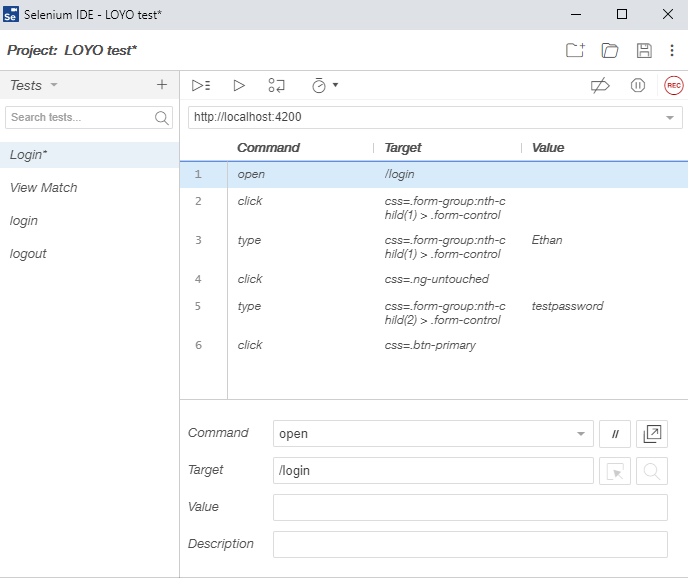
\includegraphics[width=10cm,height=5.3cm,keepaspectratio]{img/Selenium.png}
\end{center}
\section{The Elo System}
The Elo rating system, developed by Arpad Elo, is used for calculating relative skill levels of players in games such as chess.\cite{glickman1999rating} A rating is a number normally between 0 and 3000, this number changes depending on the outcomes of games. When a players rating is unknown, the score for a player is assumed to be:
\[ E_a = \frac{1}{1+10\frac{E_a-E_b}{400}} \] \cite{pelanek2014application} A player's change in rating is calculated by the following formula where ${S_a}$ is the result of the game (${Win = 1}$ and $Loss = 0$), $R_o$ is the old rating and $R_n$ is the new rating.
\[ R_n = R_o + K(S_a - E_a) \]


{\raggedright The size of the score change is determined by a dynamic K value. Initially, this K value is big (30 for their first 30 games) resulting in rapid changes in Elo. This is so a player can quickly find his or her correct place in the ranking system. As the number of games increases the K value is reduced to prevent dramatic changes in Elo.}\newline
\cite{glickmanrating} The value K used to take on the values 32, 24 or 16, depending on a player’s pre-event rating. K Factor can also be defined through this equation, where $N_i$ is the effective number of games, and m is the number of games the player completed in the game.
\paragraph{Example} If Player $E_a$ has a rating of 1200 and Player $E_b$ has a rating of 1000 with both having a K value of 30, Player $E_a$ is expected to win. If Player $E_b$ wins, the rating for player $E_b$ will increase more compared to if $E_a$ won because its rating is higher.\vfill

\chapter{System Design}
\begin{center}    
	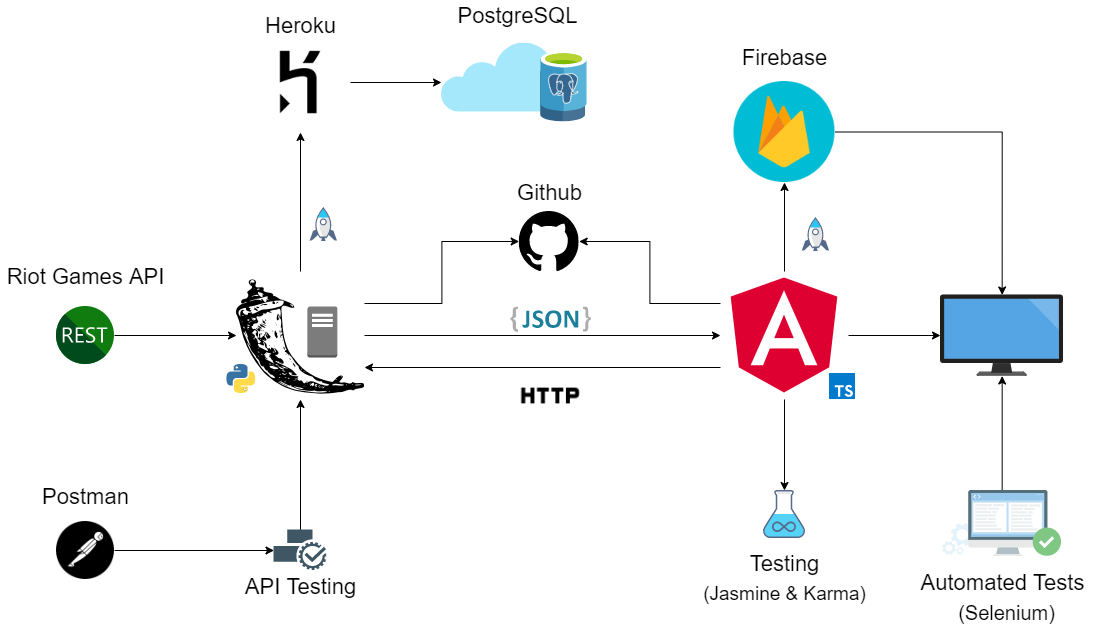
\includegraphics[width=\textwidth,height=\textheight,keepaspectratio]{img/Architecture.png}
\end{center}
As many pages as needed.
\begin{itemize}
	\item Architecture, UML etc. An overview of the different components of the system. Diagrams etc… Screen shots etc.
\end{itemize}

\begin{table}[h]
	\centering
	\begin{tabular}{x{2cm}p{3cm}}
		\toprule \\
		Column 1 & Column 2 \\
		\midrule \\
		Rows 2.1 & Row 2.2 \\
		\bottomrule
	\end{tabular}
	\caption{A table.}
	\label{table:mytable}
\end{table}

\chapter{System Evaluation}
As many pages as needed.
\begin{itemize}
	\item Prove that your software is robust. How? Testing etc. 
	\item Use performance benchmarks (space and time) if algorithmic.
	\item Measure the outcomes / outputs of your system / software against the objectives from the Introduction.
	\item Highlight any limitations or opportuni-ties in your approach or technologies used.
\end{itemize}

\chapter{Conclusion}
About three pages.

\begin{itemize}
	\item Briefly summarise your context and ob-jectives (a few lines).
	\item Highlight your findings from the evalua-tion section / chapter and any opportuni-ties identified.
\end{itemize}

